\section{生成结果的核验}
\label{sec:sgen-checks}

一个生成程序写好之后，怎样确认它给出的是想要的东西？前面几节其实已经区分了两类要核对的性质：直接生成要核对每个样本的分布及样本之间的独立性，链式更新要核对目标是否为不变分布以及链能否走遍目标。此外，实际程序与数学方法之间还隔着停止规则、有限精度和数值近似，它们各自会引入偏差。本节逐项说明怎样核对，以及经验检查能说明什么、不能说明什么。

\paragraph{直接生成：分布与独立性}
直接生成的正确性有完整的数学判据：输出分布满足式~\eqref{eq:sgen-correct-law}。前几节对每种方法都给出了这样的证明，核验时要逐条对照证明用到的条件是否在程序中成立，例如分位数是否对所有$u$有误差界、包络常数是否真正满足式~\eqref{eq:sgen-envelope}、混合采样的两步是否使用了不同的随机数。

独立性来自输入：每个样本只使用自己的一组基础随机数，组与组互不重叠。核对时要看程序是否在样本之间共用了状态，例如为了“节省”而把上一个样本剩余的随机数或中间结果留给下一个样本。只要输入不重叠，同分布且独立就有保证，样本个数再多也不会产生相关。

\paragraph{链式更新：不变性、可达性与相关性}
链的不变性同样可以证明，并且可以对小问题做精确的数值核对。把程序中的接受规则原样用在一个有限状态的小目标上（例如第~\ref{sec:sgen-mh}节的三状态目标），按程序逻辑写出完整的转移矩阵$\bm{K}$，直接计算$\pi\bm{K}-\pi$。它应在舍入误差以内为零。这种核对不依赖任何模拟，能发现遗漏建议比、遗漏拒绝时的重复记录之类的错误：前面已经算出，遗漏建议比会把不变分布变成$(2/15,2/3,1/5)$。

可达性无法用这种方式核对，它是关于整个目标支持的全局性质，要从目标的结构论证，例如说明建议分布能以正概率从任一点走到任一个正概率区域附近。第~\ref{sec:sgen-mh}节与第~\ref{sec:sgen-gibbs}节的两个反例都是每一步都正确、整体却走不通的情形。

即使链从目标分布出发，各个状态的边缘分布都是$\pi$，状态之间也一般相关，不能当作独立样本。图~\ref{fig:sgen-checks}(c)是二元高斯Gibbs采样中$X_1$的样本自相关，与第~\ref{sec:sgen-gibbs}节算出的$\rho^{2k}$一致：$\rho=0.99$时相隔$40$轮仍有约$0.5$的相关。相关性对积分误差的影响是下一章的内容，这里只需记住：链的输出不满足独立样本的假设。

\paragraph{停止规则带来的偏差}
理论上的方法常常假设可以无限地做下去，程序却必须停下来，停止的方式会改变输出分布。

拒绝采样理论上试到接受为止。若程序为了限制时间，最多试$T$次，全部失败时返回最后一个候选，输出就不再服从$\pi$。记接受率为$a$，前$n-1$次失败、第$n$次接受的概率是$(1-a)^{n-1}a$，接受的样本服从$\pi$；$T$次全部失败的概率是$(1-a)^{T}$，此时返回的候选服从“候选在被拒绝条件下”的分布。由定理~\ref{thm:sgen-rejection}的计算，候选被拒绝且落在$A$中的概率是$\int_{A}q-\tfrac1M\int_{A}\widetilde{p}$，记其条件分布为$R$。于是输出分布为
\begin{equation}
  \bigl(1-(1-a)^{T}\bigr)\,\pi+(1-a)^{T}R .
  \label{eq:sgen-capped-rejection}
\end{equation}
偏差的权重$(1-a)^{T}$随$T$几何下降，但永远不为零。以$\operatorname{Beta}(2,2)$的例子计算，$a=2/3$，$R$的密度为
\[
  \frac{1-4x(1-x)}{1/3}=3(1-2x)^{2}.
\]
$T=1$时式~\eqref{eq:sgen-capped-rejection}给出$\tfrac23\cdot6x(1-x)+\tfrac13\cdot3(1-2x)^{2}=1$，即输出就是建议分布本身，这与“只试一次就交出候选”的直觉一致（图~\ref{fig:sgen-capped-rejection}）。

\begin{BookInlineFigure}
  \centering
  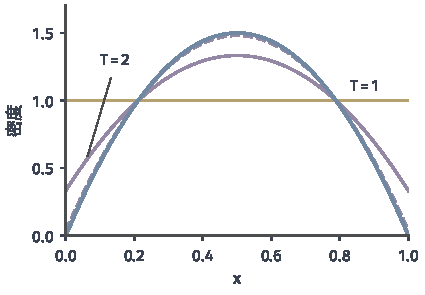
\includegraphics[width=72mm]{figures/07-probability/08-sampling-and-integration/matplotlib/sgen-capped-rejection/figure.pdf}
  \caption{最多试$T$次的拒绝采样的输出密度，目标$\operatorname{Beta}(2,2)$，建议$\operatorname{Unif}(0,1)$，$M=1/4$。黄线$T=1$（等于建议分布），紫色实线$T=2$，紫色虚线$T=4$，蓝线是目标$6x(1-x)$。偏差权重为$(1/3)^{T}$。}
  \label{fig:sgen-capped-rejection}
\end{BookInlineFigure}

链式更新也有同样的问题。从$\mu_0$出发运行$t$步，$X^{(t)}$的分布是$\mu_0K^{t}$，一般不等于$\pi$。第~\ref{sec:sgen-invariance}节的三状态例子从状态$1$出发，$5$步后的分布是$(0.219,0.5,0.281)$，离$\pi=(0.2,0.5,0.3)$还有可见的差距。“等到轨迹看起来稳定再开始记录”是一种依赖于已生成数据的停止规则，它本身也会改变被记录状态的分布。这些偏差有多大、怎样控制，是下一章讨论链初值影响时的主题。

\paragraph{有限精度与数值近似}
每一种数值近似都在数学方法与程序输出之间插入了一个误差，核验时要逐个列出。逆变换中的数值反演按引理~\ref{lem:sgen-inversion-error}改变输出的分布函数，误差界必须对全部$u$成立；协方差因子的舍入误差改变输出的协方差。链式更新中，接受比值若直接用密度相除，可能出现下溢后的$0/0$，应改用对数。Hamilton采样中步长超过稳定范围时轨道发散，表现为能量差变成很大的数或非数值，程序应把它作为拒绝处理并报告，而不是悄悄跳过这一步：跳过等于改变了转移核。

这些近似之外，还有基础随机数本身与理想模型的差距（第~\ref{sec:sgen-uniform}节）。近似生成造成的偏差不会随样本数增加而消失，它与样本数决定的随机波动是两种不同的误差，下一章将分开评价。

\paragraph{经验检查的作用与边界}
直方图、样本矩、自相关与轨迹图是最常用的经验检查。它们能发现问题，却不能证明正确。图~\ref{fig:sgen-checks}给出三种情形。

\begin{BookInlineFigure}
  \centering
  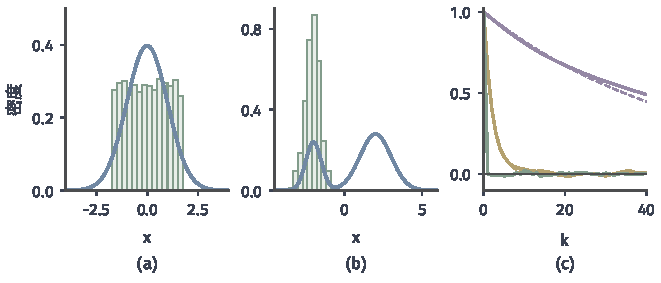
\includegraphics[width=112mm]{figures/07-probability/08-sampling-and-integration/matplotlib/sgen-checks/figure.pdf}
  \caption{经验检查能看出什么。(a)$\operatorname{Unif}(-\sqrt3,\sqrt3)$的$5000$个样本（种子$14$），样本均值$0.006$、方差$1.007$，与$\mathcal{N}(0,1)$（蓝线）的前两阶矩相同，直方图却明显不同；(b)第~\ref{sec:sgen-mh}节步长$0.3$的随机游走Metropolis的前$1000$个状态，直方图是一个干净的单峰，蓝线是混合目标；(c)二元高斯Gibbs采样中$X_1$的样本自相关（$20000$轮，种子$15$），黄线$\rho=0.8$，紫线$\rho=0.99$，虚线是$\rho^{2k}$，绿线是独立样本。}
  \label{fig:sgen-checks}
\end{BookInlineFigure}

(a)说明低阶矩相符不能说明分布正确：均匀分布$\operatorname{Unif}(-\sqrt3,\sqrt3)$的均值为$0$、方差为$1$，与标准高斯相同。若某个“高斯生成器”实际输出的是它，只检查均值与方差永远发现不了，直方图则一眼可见。反过来，直方图只比较到分箱的分辨率，比分箱更细的偏差（例如第~\ref{sec:sgen-transform}节固定轮数二分法造成的离散化）以及远处尾部的偏差，直方图也看不出来。

(b)说明经验检查只能看到已经访问过的区域。链的前$1000$个状态全部在左峰附近，直方图形状规则，与左峰的密度相符；单看这批状态，没有任何迹象提示右边还有一个占$70\%$质量的峰。只有事先知道目标有两个峰，才能看出问题。同理，从不同初值出发的多条链若都没有找到某个区域，它们彼此一致也不能说明那个区域不存在。

(c)说明自相关可以量出链的“记性”有多长，却不能说明链已经走遍了目标：一条困在单峰中的链，在峰内的自相关可能很快衰减。

所以经验检查的作用是排除明显的错误：它们发现的偏差是真实的，没有发现偏差则不构成证明。正确性的依据仍是前面各节的证明，加上对可达性的结构论证；经验检查在此基础上补充核对程序是否忠实地实现了证明中的方法。
